\chapter{细电子注是怎样得到的?}

行波管是利用电子注与高频电场之间的持续相互作用来实现微波信号放大的一种器件。因此,首先要解决的问题就是如何得到一束符合要求的电子注。实际上,从某种意义上说,行波管的工作过程就是电子注产生、成形、维持和消失的过程。从电子注角度来看,行波管可以分为下面四个区,如图\ref{ch6-1}所示。

\begin{figure}[phtb]
	\centering
	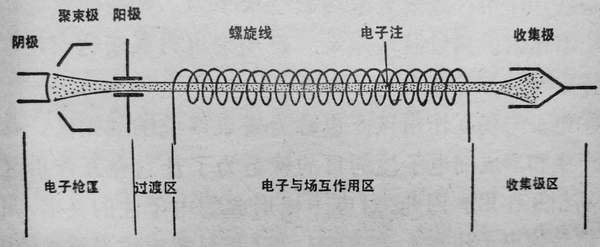
\includegraphics[width=0.65\linewidth]{figure/ch6-1}
	\caption{行波管中的电子注}
	\label{ch6-1}
\end{figure}

\begin{enumerate}
	\item 电子枪区:在此区,电子枪产生电子注并使它基本成形。这个任务是由阴极、聚束极和阳极来完成的。从阴极发射出来的电子在这三个电极产生的静电场和电子注本身空间电荷力的作用下形成一束高速细电子注(可以认为前者将使电子注会聚后者使电子注发散),并从阳极孔射出,这个情况好像子弹从手枪中射出来一样。因此,人们给这种形成和射出电子束的部件起了一个名字,叫做电子枪。	
	
	顺便提一下空间电荷力,它实际上就是电子注内电子与电子之间的相互作用力。我们知道,电子与电子之间存在着互相排斥的作用力,它们之间的距离越近,这种排斥力就越大。因此,当许多电子汇集在一起形成细电子注时,它们之间就会产生较强的排斥力,我们称之为空间电荷力,它将使电子注散开,因而是不利的因素。
	\item 过渡区。这是电子枪区和互作用区之间的中间区域。在电子枪区,作用于电子注的会聚力是静电场产生的,而发散力则是电子注中空间电荷产生的。从阴极出来的电子在这两种力的作用下形成了我们所需要的高速细电子注。在互作用区,作用于电子注的发散力依然是电子注的空间电荷力,但是会聚力却变成了磁场聚束力(详见第\ref{ch7}章)。过渡区的情况介于二者之间,在这里,电子枪电极建立的静电场急剧减小,取而代之的则是从互作用区延续过来的磁场聚束力,而空间电荷发散力则继续起作用。到过渡区末端,磁场聚束力逐渐达到互作用区中那样大小,细电子注也已成形。
	\item 电子与场互作用区,也称为聚束系统的规则区。我们知道,产生和形成细电子注的目的就是为了让它在互作用区中与高频场相互作用。因此,对电子枪形成的电子注的要求,归根到底也就是使电子注在互作用区(细而长的螺旋线慢波系统)中能够很好地同高频场持续相互作用。为此,我们对电子注提出这样三个要求:$ a .$高速:电子注应具有较高的速度,以便具备足够的动能与高频场交换。$ b. $细束:在厘米波段,螺旋线的平均直径一般是2\textasciitilde3毫米,因此要求电子注的直径约在1\textasciitilde2毫米以内。$ c. $层流特性好(关于层流特性,在本章后半部分介绍)。
	
	关于互作用区的情况,我们将在第七章中专门进行分析。
	\item 收集极区。在这个区域内,与高频场作用完毕的电子将被专门的收集极所收集,电子注在此区域内消失。
\end{enumerate}


\section{电子枪的分类}

我们知道,在普通三极管中没有电子枪,这是因为对其电子流的形状和尺寸要求并不严格,只要能得到一定的阳极电流以便在栅阳空间中与交变电场进行能量交换就可以了,它的电子流形状如图\ref{ch6-2}所示。但是,在速调管、行波管以及示波管、显象管等类电子管中,对电子流(这里应称为电子束或电子注)的形状甚至尺寸都有比较严格的要求。怎样得到一束尺寸符合我们要求的规则的电子束呢?我们利用多个电极产生的静电场来使电子束成形,以满足我们的要求。这多个电极便组成了一把电子枪。

\begin{figure}[phtb]
	\centering
	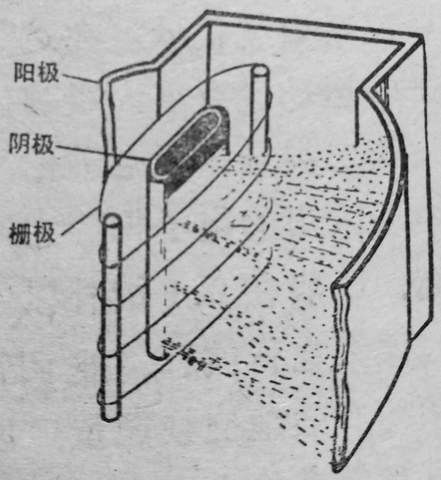
\includegraphics[width=0.3\linewidth]{figure/ch6-2}
	\caption{三极管内电子流示意图}
	\label{ch6-2}
\end{figure}


最简单的电子抢是由三个电极(阴极、聚束极和阳极)所组成的,图\ref{ch6-3}所示的两把电子枪就是这样。随着管子对电子束要求的不断提高,出现了许多种电子枪。但是,我们可以根据电子束的强度把它们分成两大类。由于导流系数很好地表示了电子束的强度,因此,常常用导流系数来区分这两类枪。

第一类是细束电子枪(或弱流电子枪),它产生低强度的电子束。显象管、示波管中采用的就是这类枪。它的特点是导流系数很低(一般在千分之一微朴以下),电子束直径很小(只有0.1\textasciitilde0.5毫米左右,因而称为“细束”)。在这类管子中为了在荧光屏上得到亮度高、直径小的光点,电子束的加速电压都很高(近万伏甚至更高,因为荧光屏的亮度将随电子束动能的增加而增大),而电子束的电流都很小(如显象管的电流约100\textasciitilde1000微安,示波管的电流约10\textasciitilde100微安。由于电流很小因此很便于用偏转电压或偏转线圈来控制它的运动以便在荧光屏上方便地得到和电信号相对应的图象或曲线),因此它的导流系数就很低。在这类低强度的电子束中,空间电荷力对电子的运动没有重大影响,因此可以忽略空间电荷的作用。

第二类是强流电子枪,这就是行波管、速调管等微波电子管中所采用的电子枪。它产生高强度的电子注,其导流系数比较高,一般在0.1微朴以上,有的高达几微朴。这是什么原因呢?原来在行波管、速调管等微波电子管中,为了使电子注和高频均有效地交换能量,以便得到足够大的功率增益,常常希望有足够多的电子参予作用,因而这些管子的电流都比较大一般都在几十毫安以上,有的甚至在几百毫安以上。可见,要比细束枪的电流大得多,故称为强流电子枪。另一方面,为了改善管子的高频性能、提高效率,我们常常希望电子注电压不要太高,对于中小功率行波管来说,通常在1000\textasciitilde3000伏之间。上面两个方面的原因使得强流枪电子注的导流系数比细束枪电子束的导流系数大得多。在强流枪产生的电子注中,电流密度都很大,因此空间电荷力的影响严重,它是使电子注向外发散的最主要原因。可见,导流系数实际上也表征了电子注内空间电荷力的大小。

\section{行波管电子枪的构造}



\subsection{会聚状电子注}



\begin{figure}[phtb]
	\centering
	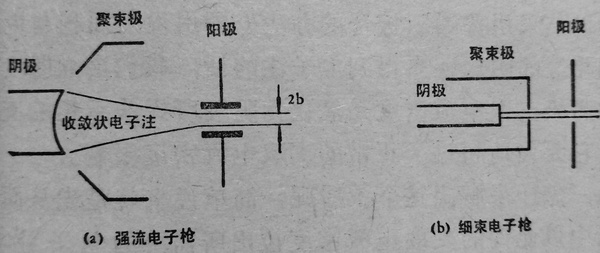
\includegraphics[width=0.65\linewidth]{figure/ch6-3}
	\caption{电子枪结构示意图}
	\label{ch6-3}
\end{figure}

图\ref{ch6-3}(a)是一把行波管电子枪的结构示意图。它是由凹球面状的阴极、漏斗状的聚束极和中心带孔的阳极组成的。我们首先来看看阴极。为什么阴极的面积要比电子注截面面积大很多呢?原来各种阴极都有一定的支取电流密度限制(如氧化物阴极的支取电流密度通常要求在200 mA/cm$ ^2 $以下),如果超过这个限制,就要使阴极的负担过重,因而其寿命将大大缩短。在普通三极管中,通常不会出现阴极支取电流密度超过限制的情况,例如某三极管,其阳极电流为25 mA,阴极面积为0.24 cm$ ^2 $,因此阴极支取电流密度为$ \frac{25}{0.24} =104$ mA/cm$ ^2 $。由于电子流截面面积和阴极面积近似相等,因此三极管中的电子流密度是和阴极支取电流密度近似相等的。但是,在行波管中,情况就大不一样了。如前所述,为了得到尽可能高的增益,常常需要较大的电子注电流(一般为几十毫安)。但是,电子注的直径却受到细长的螺旋线的限制。我们知道,螺旋线的直径是由工作频率、电子注电压等决定的般为2\textasciitilde3毫米。因此,电子注的直径被限制在1.8毫米以下($ \frac{b}{a} $以0.6计)。可以算出,其电子注电流密度是很大的(例如,某行波管的电子注电流为25毫安,而电子注直径仅1毫米因此,其注电流密度高达3.18 A/cm$ ^2 $),这是一切强流电子器件的共同特点。


如果仍然采用普通三极管的办法(即用发射面积与电子流截面面积相等的阴极)来得到电子注的话,我们会立即发现这样高的阴极支取电流密度是氧化物阴极所无法承担的支取电流密度,它大大地超过了正常的支取电流密度限制。

那么,怎样来解决这个矛盾呢?简单说来就是先从面积较大的阴极中以允许的支取电流密度拉出所需要的电子注电流$ I_0 $,然后想办法把它压缩到所要求的电子注截面尺寸。由于互作用区螺旋线的横截面是圆形的,在它上面传播的高频场都是轴对称的,因此与它交换能量的电子注也应当是圆形截面的。

怎样利用压缩的办法来得到一个圆截面的细电子注呢?支削好笔尖的铅笔给了我们一个很好的启示。如果能够把象铅笔杆那样粗的电子注压缩成铅笔芯那样细的电子注,那么,不管铅笔芯的电流密度多么大,我们总是可以用增大铅笔杆直径的办法使铅笔杆处的粗电子注的电流密度符合氧化物阴极正常支取电流密度的要求的。这种铅笔尖式电子流的形状是会聚状或收敛状的,这就是行波管中电子注的特点。因此,我们的任务就是如何得到这种会聚状电子注。为此,我们需要先介绍一下球形二极管的一些概念。

\subsection{球形二极管}

\begin{figure}[phtb]
	\centering
	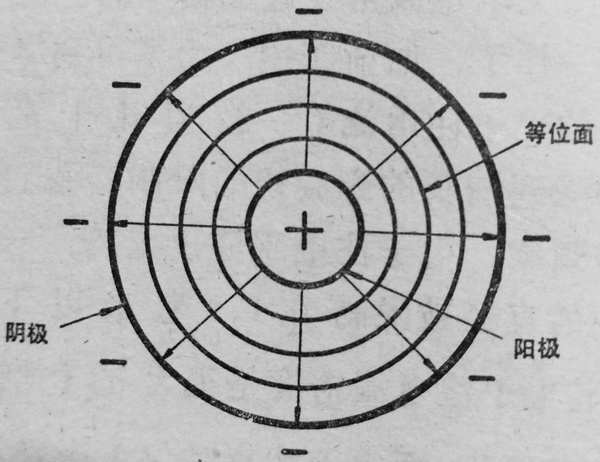
\includegraphics[width=0.42\linewidth]{figure/ch6-4}
	\caption{球形二极管电场分布示意图}
	\label{ch6-4}
\end{figure}

\begin{figure}[phtb]
	\centering
	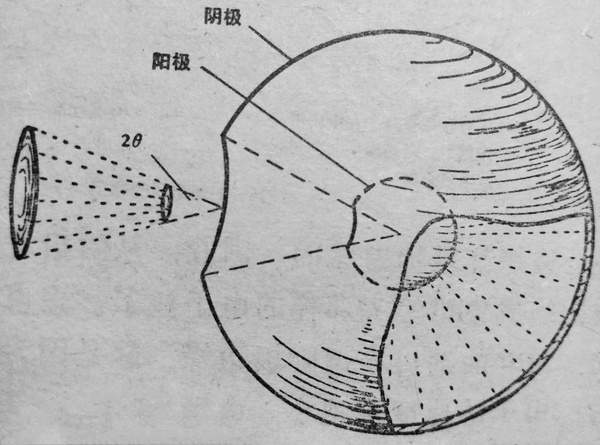
\includegraphics[width=0.5\linewidth]{figure/ch6-5}
	\caption{从球形二极管中取出一个圆锥形二极管}
	\label{ch6-5}
\end{figure}

球形二极管是一个假想的二极管,它的结构如图\ref{ch6-4}所示。它是由两个同心球面电极构成的,外边大球的内表面为阴极,其上涂有发射材料,里面的小球是阳极,如果在两个电极上加上直流电压,它们之间就会产生球对称的辐射状电场,如图所示。在这个辐射电场的作用下,外球面(阴极)发射的电子就将沿着电力线射向内球面(阳极),从而形成了球对称的、会聚状的电子注。我们可以进一步设想,如果能够从球面二极管中挖出来一部分,使得它的外形像一个圆锥那样,如图\ref{ch6-5}所示,那么,它的电子流形状就和铅笔尖的形状很相像了。此时,阴极和阳极将是两个同心球面的一部分。这就是我们为什么要把阴极做成凹球面状的原因。聚束极的作用是什么呢?可以想象,只靠凹球面状阴极我们所能得到的,并不是会聚状的电子流而是象图\ref{ch6-6}(a)所示的向外发散的电子注,这是由于空间电荷排斥力造成的。由于这种空间电荷排斥力的影响,电场将发生畸变,电力线要发生弯曲,这种现象在电极边缘尤为严重(如图\ref{ch6-6}(a)所示)。我们知道,电子是在电力线所表示的电场作用下运动的,如果电力线发生弯曲,那么,电子注的形状也就要发生畸变,因而不能满足我们的要求。为了改变电极边缘附近的电场,使它符合我们的要求,人们经过计算和模拟,设计出一种电极,即所谓聚束极,通常它是一个轴对称的电极,在它的上面加上一定的电压以后,聚束极将对电场进行修正,使得阴极和阳极之间的电场,不论中间还是边缘都是辐射状的。因此,从阴极发射出来的电子注就能被压缩成象铅笔尖那样的电子注了。聚束极常常被做成漏斗状的,漏斗的细口靠近阴极边缘,这是因为离阴极表面越近的地方,电子的速度就越小,电子的密度比较大,空间电荷的排斥力也比较大,电子注向外发散的趋势也强一些,因此,要求聚束极离阴极近些,以便对电子注施加较大的会聚力。理论计算得到,聚束极的漏斗斜面应当与电子注边缘成$ \ang{67.5} $的夹角才能保证电子注有良好的会聚形状。为了使用和生产方便起见,聚束极的电位常常和阴极相同,但也有比阴极电压稍高或稍低的,这要由不同的设计要求来决定。

\begin{figure}[phtb]
	\centering
	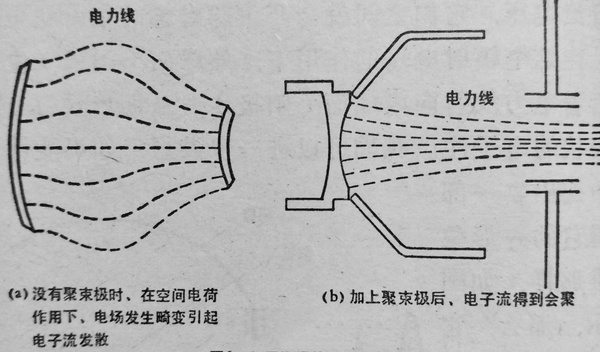
\includegraphics[width=0.75\linewidth]{figure/ch6-6}
	\caption{聚束极的作用}
	\label{ch6-6}
\end{figure}

对于阳极的形状,是这样考虑的:我们分析球面二极管并导出圆锥二极管并不是单纯为了设计一个圆锥二极管,而是要得到一束铅笔尖状的电子注。因此,阳极中心必须开孔,以便让电子注通过。阳极中心开孔对于电子枪区的电场略有影响(所谓阳极孔效应),但是通常不大。由于阳极对电子枪区电场的影响要比聚束极小得多,因此,为了加工方便起见,阳极不必做成球面状,常常做成一个中心开孔的圆片镶上一段小圆筒,如图中所示。或者干脆只做成一个中心开孔的圆片,中心孔附近略微有些斜面状就可以了。

这样由凹球面状的阴极、漏斗状的聚束极和中心开孔的圆片状阳极组成的电子枪就能够成功地得到铅笔尖状的会聚电子注,并达到高速细束的要求。

顺便提一点,细束电子枪的阴极面是一个不大的平面,聚束极是一个顶部中心开孔的中空圆筒,如图\ref{ch6-3}(b)所示。这是因为细束电子枪电子注电流很小的缘故。细束枪电子注内的空间电荷影响很小,通常可以忽略。

\section{怎样得到一把好的电子枪}

从前面的分析中我们知道,在行波管中,为了得到符合要求的强流电子注,常常采用轴对称收敛注电子枪,这种电子枪有下列优点:
\begin{enumerate}
	\item 收敛注电子枪能得到比阴极发射密度大得多的注电流密度,因此很容易满足行波管对电子注的要求。 
	\item 收敛注电子枪的阴极负荷较轻,因此,有利于延长阴极的寿命。
	\item 收敛注电子枪得到的电子注横向速度较小,因而使电子注聚束所需的磁场较小
\end{enumerate}

\subsection{对电子枪的基本要求}

对电子枪的基本要求归纳起来有下面几点:
\begin{enumerate}
	\item 电子注电流和电压(阳极电压)或导流系数应满足高频系统提出的要求。阳极上截获的电流越小越好。
	\item 电子注直径应满足高频系统提出的要求。因为高频系统决定后螺旋线的尺寸也就定了,因此电子注的直径便可决定。
	\item 电子注进入聚束磁场时应尽可能与轴线平行,电子注的层流特性要好。
	\item 工艺上容易实现,结构要牢靠。
\end{enumerate}

\subsection{电子枪的参量}

实际的电子枪是如何满足这些基本要求的呢?在回答这个问题之前,我们再来看一下在第\ref{ch4}章中提到的电子枪的导流系数$ P_\theta $。

我们知道,任何电子枪,如果画出它的伏安(阳极电压\textasciitilde 电子注电流)特性的话,都服从一条共同的规律:电流与电压的二分之三次方成正比。这个规律,我们称它为二分之三次定律,它的数学表达式是:
\begin{equation} \label{eq:ch6-1}
	I=P_\theta U^{3/2} \qquad\textrm{或}\; P_\theta = \frac{I}{U^{3/2}}
\end{equation}

式中:导流系数$ P_\theta $是一个常数,在电子枪的结构确定以后,导流系数也就定了。

导流系数有什么物理意义呢?

\begin{enumerate}
	\item 导流系数表征了电子枪在一定加速电压下给出电流的能力。$ P_\theta $越大,则在同样加速电压下,电子枪产生的电子注电流就越大;或者在同样电子注电流下,所需的加速电压就越低。$ P_\theta $对行波管许多重要指标,如增益、功率、效率等都有重大的影响,因此是电子枪最重要的参量。提高导流系数往往是改进行波管的一条重要途径
	\item 导流系数表征了电子枪中空间电荷作用的程度。$ P_\theta $越大,表示在同样电子注电压下电子注电流越大,也就意味着电子注中空间电荷密度$ \rho $越大,因此,形成锥形电子注所遇到的困难也越大。当$ P_\theta > 1$微朴后,空间电荷密度很大:各种矛盾将要激化,必须考虑更多的因素,对电极作各种修正。因此,高导流系数的电子枪的结构就比较复杂。我们常常把强流电子枪按$ P_\theta $的大小分成两大类:$ P_\theta =0.1\textasciitilde 1$微朴,称为低导枪。中、小功率行波管中多用这种枪,它的结构比较简单。$ P_\theta =1\textasciitilde 2$微朴或更大,称为高导枪。多用于大功率行波管或其它微波管中,结构比较复杂。
	\item 导流系数还表征了电子枪的结构情况与尺寸大小。$ P_\theta $大,阴极与阳极距离一定较近。$ P_\theta $大,电子注半锥角$ \theta $一定较大,即阴极直径较大。 
\end{enumerate}

对于本书重点介绍的行波管,其电子枪导流系数都很低因此可以采用结构比较简单的低导枪。典型的低导枪结构如图\ref{ch6-7}所示。它们的结构尺寸是怎样确定的呢?

\begin{figure}[phtb]
	\centering
	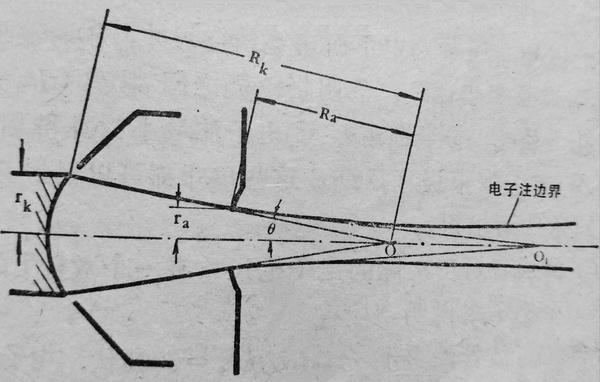
\includegraphics[width=0.65\linewidth]{figure/ch6-7}
	\caption{典型的低导枪结构示意图}
	\label{ch6-7}
\end{figure}


一个管子的高频系统设计完毕以后,电子注电压$ U_0 $、电子注电流$ I_0 $和电子注半径$ r_b $就知道了。于是我们可以算出它的导流系数$ P_\theta = \frac{I_0}{U^{3/2}} $

若阴极面半径为$ r_K $,那么阴极的支取电流密度就是$ J_K = \frac{I_K}{\pi r_K^2} $,式中阴极电流$ I_K$即电子注电流$ I_0 $(假定阳极电流等于零)。我们可以根据阴极的性能选择一个合适的$ J_K $值(例如200 mA/cm$ ^ 2$),于是由公式$ r_K = \sqrt{\frac{I_K}{\pi J_K}} $便可决定阴极面半径。

根据$ r_K $和$ r_b $我们可以求得电子枪的面压缩比$ M_{\textrm{面}} $,这是电子枪的另一个参量,它的定义是电子注电流密度与阴极电流密度之比,因此有:
\begin{equation} \label{eq:ch6-2}
	M_{\textrm{面}} = \frac{\left(\frac{I_K}{\pi r_b^2}\right)}{\left(\frac{I_K}{\pi r_K^2}\right)} = \frac{r_K^2}{r_b^2}
\end{equation}
面压缩比表征了电子注的收敛程度。我们还常用到线压缩比$ M_{\textrm{线}} $,$ M_{\textrm{线}} $定义为:
\begin{equation} \label{eq:ch6-3}
	 M_{\textrm{线}}  = \frac{r_K}{r_b}
\end{equation}

除此以外,还要确定下面这些结构尺寸:(1)阴极曲率半径$ R_K $,(2)阳极曲率半径$ R_a $,(3)阴极阳极之间距离($ R_K-R_a $)(4)阳极孔半径$ r_a $,(5)半锥角$ \theta $,(6)电子注最小截面和阳极之间的距离$ Z_{\textrm{min}} $,(7)聚束极直径$ D_g $。这些尺寸都可以根据$ P_\theta $、$ r_b $、$ r_K $等已知条件而求得。

为了使读者对于实际的电子枪尺寸有一个数量上的概念我们举一个例子来说明。

已知某行波管的电子注电压为$ U_0 = 3000 $\,V,电子注电流为$ I_0 = 25 $\,mA,电子注半径为$ r_b = 0.55 $\,mm。我们来计算其电子枪尺寸。

\begin{enumerate}
	\item 算出导流系数$ P_\theta $。
	\begin{equation*}
		P_\theta = \frac{I_0}{U_0^3/2} = 0.153\,\textrm{微朴}
	\end{equation*}
	可见,它的导流系数很低,是低导枪。
	\item 确定阴极半径$ r_K $。
	采用氧化物阴极,选取其支取电流密度为$ J_K = 150 $毫安/厘米$ ^2 $,则可算得:
	\begin{equation*}
		r_K = \sqrt{\frac{I_0}{\pi J_K}} = 0.23\,\text{cm} = 2.3\,\textrm{mm}
	\end{equation*}
	取$ r_K = 2.5 $毫米,即直径$ d_K = 5 $毫米。
	\item 求出压缩比。
	
	面压缩比$ M_{\textrm{面}} = \dfrac{r_K^2}{r_b^2} = \left(\dfrac{2.5}{0.55}\right)^2 = 4.55^2 = 20.7$
	
	
	线压缩比$ M_{\textrm{线}}  = \dfrac{r_K}{r_b} = 4.55 $
	
	一般认为,随着压缩比和导流系数的增加,阴极发射不均匀程度和电子注中非层流性将增加,电子注的形状尺寸对阴极表面发射情况的变化也越敏感,容易产生散焦(关于散焦,下章将讲到)。因此对于长寿命行波管,我们要求:面压缩比$ M_{\textrm{面}} < 25\textasciitilde 30$,导流系数$ P_\theta < 0.3 $微朴。
	\item 确定收敛半角$ \theta $(即半锥角)。
	
	选用氧化物阴极,取其工作温度$ T_K =\SI{750}{\degreeCelsius}= \SI{1023}{\kelvin} $,算出$ \sqrt{\frac{U_0}{T_K}} $。由$ \sqrt{\frac{U_0}{T_K}} $和$ M_{\textrm{线}}$查曲线得到$ \frac{R_K}{R_a }= 2.64$。由公式算得$ \theta =\SI{11}{\degree}\SI{6}{\arcminute}$。
	\item 确定阴极曲率半径$ R_K $。
		\[ R_K = \frac{r_K}{\sin \theta} = 13\,\textrm{mm} \]
	\item 求出阳极曲率半径$ R_a $和阳极孔半径$ r_a $。
	
	由$ \frac{R_K}{R_a} = 2.64$可求得$ R_a = \frac{R_K}{2.64} = 4.92$\,mm。
	
	$ r_a = R_a\cdot\sin\theta \approx1\,\textrm{mm} $,扩孔15\%,取$ r_a=1.15 $\,mm。
	\item 求出阴极与阳极之间的距离$ (R_K-R_a) $。
	
	$ R_K-R_a=13-4.92\approx 8.1 $\,mm。
	\item 求出电子注最小截面和阳极之间的距离$ Z_\textrm{min} $。
	
	查曲线后算得$ Z_\textrm{min}\approx 10 $\,mm。
	\item 聚束极直径$ D_g $取11.6毫米。
\end{enumerate}



这样,我们就把电子枪的尺寸大致确定下来了。应当指出,我们上面仅仅介绍了大致的计算步骤,计算是极粗略的在实际的电子枪设计计算中,往往要经过反复的理论计算和实验修正,才能得到一把理想的电子枪。

近年来,在电子枪的设计中已经广泛地采用了电子计算机,它可以给出精确的计算结果,并画出电子注的轨迹,从电子注轨迹中可以看出电子注层流特性是否良好。

求得了上述一系列尺寸以后,我们便可以根据这些尺寸做出电子枪来,并对它进行电参数测试,必要时还要反复修改电极尺寸和形状,最后才能得到一把符合我们要求的电子枪。


\section{两个问题}

我们在前面的叙述中曾经提到电子注的层流特性以及阳极孔效应等,它们是怎么一回事呢?

\subsection{电子的热初速}

使电子注发散的原因,除了空间电荷的排斥力外,还有电子的热初速,因此我们需要专门介绍一下。虽然空间电荷排斥力是发散的主要因素,但是当空间电荷所引起的发散力被克服以后,电子的热初速这个次要因素便突出出来了。它会影响计算的准确性,引起误差。特别是在阳极电压较低、电子注较细的情况下,这个次要因素的作用就更突出了。

所谓热初速,是指电子从热阴极发射出来时由于热运动而具有的初速度。我们知道热运动是杂乱的无规则的,因此,这些电子的运动方向(也就是速度方向)也是各不相同的。有沿轴方向的,也有沿电子注截面半径方向的(即所谓横向的热初速),后者将是引起电子注发散的一个因素。横向热初速的主要影响是:

\begin{enumerate}
	\item 横向热初速引起电子轨迹的偏离。电子的热初速都不算大,它相当于0.1伏的阳极电压所产生的速度。因此,如果是沿轴方向的,那么和一千伏以上的阳极电压比较起来是微不足道的,可以不予考虑。但是问题在于那些沿半径方向运动,或者说有径向速度分量的电子,它们的速度虽然不大,但是在飞离阴极后,由于横向速度的存在,它们就要偏离轴线向外运动,这就会影响电子注的会聚,起了附加的发散作用。在实际设计中就必须对这个由于电子横向热初速引起的轨迹偏离进行计算。
	\item 横向热初速造成电子注截面中电流密度分布的不均匀。从理想的电子枪中出来的电子注,其速度和密度都是均匀的。但是,由于电子横向热初速的存在,会使电子注的密度不均匀,同时还使原来很清晰的边界向外扩散,使边界变得模糊我们在设计电子枪时,考虑到这个因素的影响,应该把算得的电子注直径适当放大些。
\end{enumerate}

\subsection{层流特性}

我们观察小溪流水时可以发现有两种情况:一种是所谓层流”,在这种情况下,水流是很平稳的,好像分成若干层那样往前流动,它只有纵向流动而没有横向流动。另一种情况是“湍流”,此时,水流是起伏不平的,甚至有旋涡存在,这说明不仅有纵向流动而且有剧烈的横向流动。同样道理,我们希望电子枪产生的电子注也能够象层流的水流那样平稳地流动。这样,平行射入螺旋线中的电子注就能在纵向磁场的聚束下很好地与高频场交换能量。电子注层流特性好主要表现在电子没有横向运动,电子的轨迹没有交叉。如果层流特性不好电子存在着剧烈的横向运动,那么,电子就很容易打到阳极和螺旋线上去,因而和高频场相互作用的电子数就会减少。可见,改善电子注的层流特性是很重要的。

哪些因素会破坏电子注的层流特性呢?虽然电子横向热初速能够使层流特性变坏,但最主要的原因还是电子注的边缘电子经过阳极孔时所产生的影响。具体地说,离轴远的(电子注边缘的)电子受阳极孔的发散作用小,会聚角大,其轨迹如图\ref{ch6-8}(a)中的轨迹1;而离轴近的电子受阳极孔的发散作用大,会聚角小,其轨迹如图\ref{ch6-8}(a)中的轨迹2、3。从图\ref{ch6-8}(a)可以看到:由于阳极孔的影响,电子的轨迹发生了交叉,从而破坏了电子的层流性,在不同的电子注截面上,电流密度分布变得不均匀了。图\ref{ch6-8}(b)绘出了$ A $和$ B $两个截面上的电子的密度分布。在横截面$ A $处,电子注边缘是一个电流密度很大的圆环,而中心部分电流密度小。在横截面$ B $处,中心是一个电流密度很大的圆斑,其它地方电流密度都比较小。$ A $处和$ B $处的这两种情况,正如图中所示,是由于电子轨迹交叉引起的。实践证明,利用下面两种方法可以改善层流特性:

\begin{enumerate}
	\item 减小阴极曲率半径(即加大阴极半锥角$ \theta $)能改善电子注的层流特性。
	\item 采用阴极刮边的方法也可以改善电子注的层流特性。这是因为,电子轨迹的交叉主要是由于外层电子过于向内所造成的,所以我们很自然地会想到,把这些捣乱的外层电子去掉因此就采取了阴极刮边的办法,即将阴极边缘的发射物刮掉或者在阴极边缘嵌以无发射环。实践证明这个方法也是行之有效的。
\end{enumerate}


\begin{figure}[phtb]
	\centering
	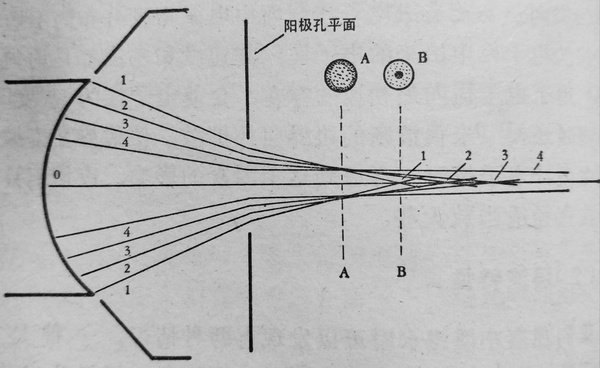
\includegraphics[width=0.85\linewidth]{figure/ch6-8}
	\caption{阳极孔对层流特性的影响}
	\label{ch6-8}
\end{figure}